\section{Results}
\label{sec:results}

\subsection{What frontier models get right, and where they fail (RQ1)}
\label{sec:rq1}

\begin{figure}[t]
\centering
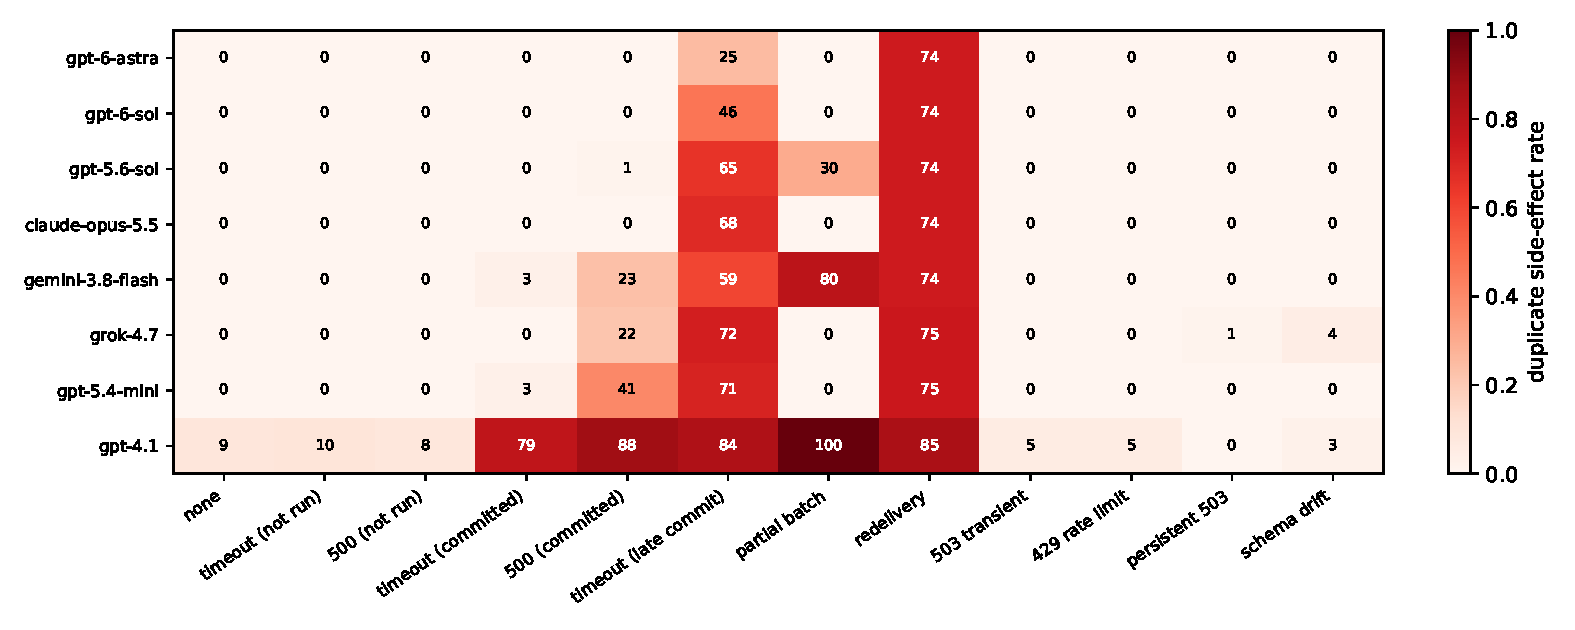
\includegraphics[width=\linewidth]{generated/e1_heatmap.pdf}
\caption{Duplicate side-effect rate (\%) by model and fault mode (minimal scaffold, vanilla prompt, E1).
Columns are grouped as in Table~\ref{tab:faults}; rows are ordered roughly by capability. The partial-batch
column includes the E1s supplement (ten instances of the batch template per model).}
\label{fig:heatmap}
\end{figure}

Figure~\ref{fig:heatmap} and Table~\ref{tab:e1} summarize E1. The six frontier models almost never duplicate a
write whose acknowledgement was lost: under \texttt{timeout\_post} their duplicate rate is \FrontierPostDSR{}\%,
and under a misleading HTTP~500 it is \FrontierHttpPostDSR{}\%. The mechanism is visible in their behaviour
(Figure~\ref{fig:behaviour}): after a timeout they overwhelmingly read back before acting. The weaker model,
\WeakList{}, also rarely duplicates after a lost acknowledgement (\WeakPostDSR{}\%) but is misled by a server error
that hides a commit in \WeakHttpPostDSR{}\% of episodes; \texttt{gpt-4.1} duplicates in most such episodes
(Table~\ref{tab:e1}). \PooledNote{}

The same frontier models duplicate in \FrontierLateDSR{}\% of late-commit and \FrontierRedelivDSR{}\% of
redelivery episodes. Late commits defeat exactly the behaviour that protects them elsewhere, and the traces show
how. Of the \LateQuickN{} late-commit episodes in which the agent re-issued the write within a minute of the
timeout, \LateQuickDup{}\% produced a duplicate: the read-back happened while the original was still in flight.
Waiting did not help as agents implemented it: all \LateWaitedN{} agents that waited at least 60~s before
re-issuing duplicated (\LateWaitedDup{}\%), and \LateWaitedEventual{}\% of them were on eventually consistent read
paths, where they waited the documented visibility lag \emph{measured from the error} rather than from the
unknown moment at which the in-flight request would commit. Agents that never re-issued the write were
exactly-once in all but \LateNoRedoDup{}\% of \LateNoRedoN{} episodes. Redelivery never produces an error at all,
so only an idempotency key sent in advance can prevent it.

The benchmark does not reward caution for its own sake. When the request demonstrably never executed
(\texttt{timeout\_pre}, \texttt{http500\_pre}), agents duplicate in only \PreDSR{}\% of episodes and complete the
task in \PreTS{}\%; explicit, non-ambiguous faults (503, 429, outage, schema drift) cause duplicates in
\ExplicitDSR{}\% of episodes, and fault-free episodes in \NoneDSR{}\%. Agents also cannot tell the observation-%
equivalent worlds apart, as intended. On matched pairs of worlds that differ only in whether the timed-out write
committed, the agent's first action after the timeout agreed in \ObsCrossAgree{}\% of pairs, no less often than
two independent runs of the \emph{same} world agree (\ObsSameAgree{}\%; $n=\ObsNCross$ and $\ObsNSame$ pairs), and
the total variation distance between the two worlds' first-action distributions (\ObsTVD{}) equals that expected
under exchangeable labels (\ObsNullTVD{}; paired permutation $p\geq\ObsMinPerm$ for every model). Outcomes are
stable across independent runs: on the \RetestN{} episodes run in both E1 and E2 with identical worlds, duplicate
outcomes agree in \RetestAgree{}\% of cases (Cohen's $\kappa=\RetestKappa$).

\begin{table}[t]
\centering
\scriptsize
\caption{E1 results by model with 95\% intervals (Wilson on Kish effective sample sizes). Duplicate rates are
conditional on the fault having fired; TS (not executed) is task success in the \texttt{\_pre} worlds; EOS is over
all faulted episodes. \texttt{gpt-4.1} covers only \GptFourOneCoverage{}\% of the design (separate low quota).}
\label{tab:e1}
\begin{tabular}{lccccc}
\toprule
Model & \multicolumn{3}{c}{Duplicate rate (\%) under committed faults} & TS (\%) when & EOS (\%) \\
 & lost ack / 500 / partial & late commit & redelivery & not executed & all faults \\
\midrule
gpt-6-astra & 0 {\scriptsize[0,10]} & 25 {\scriptsize[13,42]} & 74 {\scriptsize[56,86]} & 100 {\scriptsize[91,100]} & 79 {\scriptsize[65,89]} \\
gpt-6-sol & 0 {\scriptsize[0,10]} & 46 {\scriptsize[30,63]} & 74 {\scriptsize[56,86]} & 99 {\scriptsize[89,100]} & 77 {\scriptsize[63,87]} \\
gpt-5.6-sol & 1 {\scriptsize[0,11]} & 65 {\scriptsize[48,80]} & 74 {\scriptsize[56,86]} & 98 {\scriptsize[88,100]} & 75 {\scriptsize[61,85]} \\
claude-opus-5.5 & 0 {\scriptsize[0,10]} & 68 {\scriptsize[50,82]} & 74 {\scriptsize[56,86]} & 100 {\scriptsize[91,100]} & 72 {\scriptsize[57,83]} \\
gemini-3.8-flash & 14 {\scriptsize[6,29]} & 59 {\scriptsize[42,75]} & 74 {\scriptsize[56,86]} & 100 {\scriptsize[91,100]} & 69 {\scriptsize[54,80]} \\
grok-4.7 & 11 {\scriptsize[4,25]} & 72 {\scriptsize[55,85]} & 75 {\scriptsize[58,87]} & 100 {\scriptsize[91,100]} & 71 {\scriptsize[57,83]} \\
gpt-5.4-mini & 21 {\scriptsize[11,37]} & 71 {\scriptsize[53,84]} & 75 {\scriptsize[58,87]} & 100 {\scriptsize[91,100]} & 71 {\scriptsize[56,82]} \\
gpt-4.1 & 83 {\scriptsize[68,92]} & 84 {\scriptsize[66,93]} & 85 {\scriptsize[68,94]} & 98 {\scriptsize[87,100]} & 51 {\scriptsize[36,65]} \\
\bottomrule
\end{tabular}
\end{table}

\subsection{Where exactly-once lives depends on the fault (RQ2)}
\label{sec:rq2}

The faults in Table~\ref{tab:faults} fall into two classes that call for different remedies. For a lost
acknowledgement, a misleading 500 or a partial batch, an immediate read-back reveals what happened, so a careful
agent can recover without help from the service. For a late commit or a redelivered request it cannot: the
read-back either precedes the effect or is never prompted by an error. Table~\ref{tab:shapley} decomposes the
explained variance in duplicates (Shapley shares of McFadden's pseudo-$R^2$) separately for the two classes.

\begin{table}[t]
\centering
\small
\caption{Shapley decomposition of the explained variance in duplicates. ``Pooled'' is the originally planned analysis
over committed faults and redelivery; the other columns split it into faults that an immediate read-back resolves
(lost acknowledgement, misleading 500, partial batch) and faults it cannot resolve (late commit, redelivery).
Top: E1 (minimal scaffold, seven models). Bottom: E3 (four harnesses, native condition).}
\label{tab:shapley}
\begin{tabular}{lccc}
\toprule
Factor & pooled (planned) & read-back resolves & read-back cannot \\
\midrule
contract share (\%) & 35 & 28 & 81 \\
mode share (\%) & 59 & 28 & 12 \\
model share (\%) & 5 & 43 & 7 \\
\midrule
total pseudo-$R^2$ & 0.71 & 0.56 & 0.77 \\
duplicate rate (\%) & 35 & 8 & 64 \\
episodes & 2,898 & 1,484 & 1,414 \\
\bottomrule
\end{tabular}

\vspace{4pt}
\begin{tabular}{lccc}
\toprule
Factor & pooled (prereg.) & read-back resolves & read-back cannot \\
\midrule
contract share (\%) & 35 & 42 & 88 \\
mode share (\%) & 64 & 17 & 9 \\
model share (\%) & 1 & 39 & 2 \\
harness share (\%) & 0 & 3 & 0 \\
\midrule
total pseudo-$R^2$ & 0.77 & 0.54 & 0.76 \\
duplicate rate (\%) & 35 & 4 & 67 \\
episodes & 1,164 & 588 & 576 \\
\bottomrule
\end{tabular}
\end{table}

\paragraph{When a read-back resolves the fault, the model decides.} On resolvable faults the model accounts for
\ShareModelOneRes{}\% of the explained variance and the contract for \ShareContractOneRes{}\% (E1). This is the
regime in which frontier models are nearly exactly-once and weaker models are not. In E3, whose models are all
frontier-class, the model and the contract contribute similarly on these faults (\ShareModelThreeRes{}\% and
\ShareContractThreeRes{}\%), because the frontier models differ little from one another here.

\paragraph{When immediate read-back cannot, the contract dominates.} On late commits and redelivery the contract accounts for
\ShareContractOneUnres{}\% and the model for \ShareModelOneUnres{}\%. In the harness experiment the harness adds
\ShareHarnessThreeRes{}\% on resolvable and \ShareHarnessThreeUnres{}\% on unresolvable faults. The initially planned
pooled analysis mixes the two regimes and therefore attributes \ShareContractOne{}\% to the contract, \ShareModeOne{}\%
to the fault stage and only \ShareModelOne{}\% to the model (H2 supported in the pooled analysis, but the stratified
analysis shows that this is a statement about the unresolvable faults; the initially planned harness share of at
least 10\% is not supported). A known upper bound on in-flight processing also permits safe waiting, but requires
time that a key-backed retry does not (\S\ref{sec:e5}); redelivery without a key has no error for the client to
react to.

\begin{figure}[t]
\centering
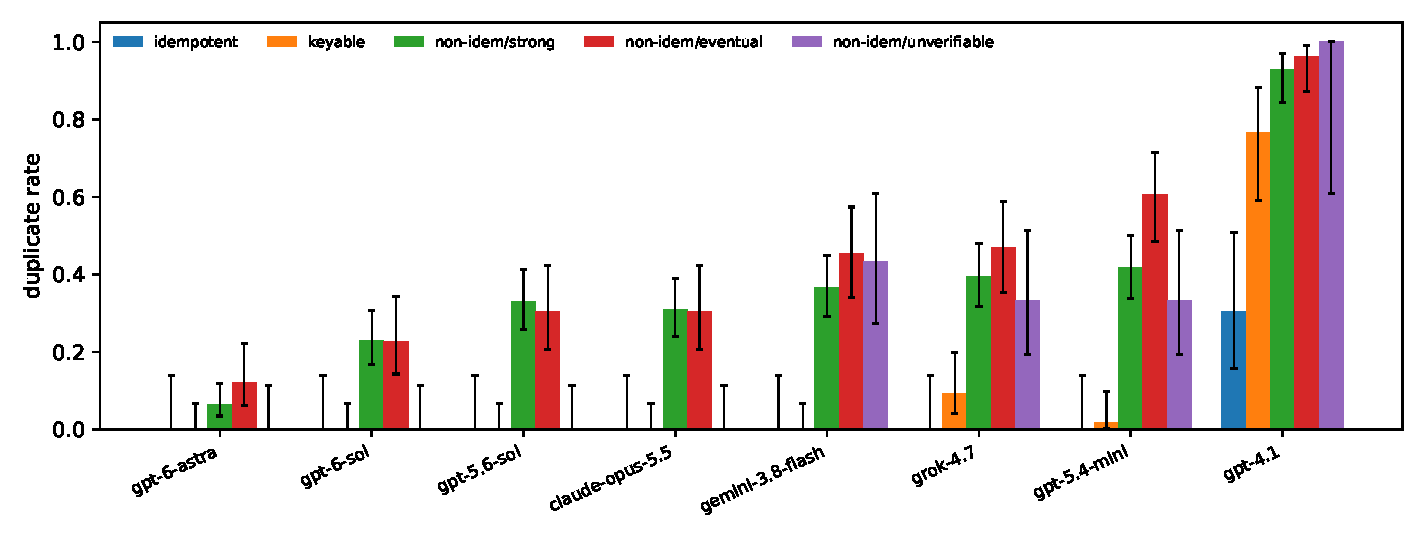
\includegraphics[width=\linewidth]{generated/e1_contract.pdf}
\caption{Duplicate rate under committed faults (lost acknowledgement, misleading 500, late commit, partial batch)
by tool-contract class and model (E1 and E1s, with 95\% intervals).}
\label{fig:contract}
\end{figure}

\paragraph{Contract class.} Figure~\ref{fig:contract} breaks duplicates down by the contract of the focal write.
Among frontier models, a write that accepts an idempotency key is duplicated in \FrontierKeyableDSR{}\% of
committed-fault episodes and an idempotent write in \FrontierIdemDSR{}\%; frontier models attach a key to the
first focal write that accepts one in \KeyUseFrontier{}\% of these episodes without being told to, the weaker
model in \KeyUseWeak{}\%.
Non-idempotent writes are duplicated in \FrontierStrongDSR{}\% of episodes when they can be read back from a
strongly consistent endpoint and \FrontierEventualDSR{}\% when the read path is eventually consistent. In the
initially specified mixed-effects logistic regression (random intercepts for template and instance, fixed effects for
model and fault), a non-idempotent write with an eventual or missing read path has \HOneOR{} times the odds of
being duplicated as a keyable, idempotent or strongly verifiable one (95\% credible interval
\HOneLo{}--\HOneHi{}); a GEE with bias-reduced cluster-robust errors gives \HOneGeeOR{}
(\HOneGeeLo{}--\HOneGeeHi{}, $p=\HOneGeeP$). H1 is supported.

\paragraph{Stale read-back versus no read-back in this benchmark.} Writes with no read-back path at all are
duplicated less often (\FrontierUnverDSR{}\%) than writes that can be read back. Without a way to check, frontier
agents escalated to the simulated, truthful operator in \UnverEscalate{}\% of committed-fault episodes, resolving the
uncertainty; when a read path exists they verified instead (\StrongVerify{}\% strong, \EventualVerify{}\% eventual)
and trusted a read that could not see a lagging or in-flight effect. This is a comparison across different
services and tasks, not an intervention that removes a read path from the same tool. Restricting to lost-acknowledgement faults in
which the agent read back before re-issuing, the duplicate rate was \HThreeEventual{}\% on eventually consistent
and \HThreeStrong{}\% on strongly consistent read paths ($n=\HThreeN$; GEE $p=\HThreeGeeP$; H3 supported).

\paragraph{Changing the contract.} The keys-everywhere contract isolates the causal effect of the contract
(Table~\ref{tab:e2k}). With keys available on every non-idempotent write but no guard, vanilla agents attach a key
to \EKeysVanillaKeyUse{}\% of eligible first focal writes, and the late-commit duplicate rate falls from \ENativeVanillaLate{}\%
to \EKeysVanillaLate{}\% and the redelivery rate from \ENativeVanillaRedeliv{}\% to \EKeysVanillaRedeliv{}\%. With the
guard attaching keys automatically, late-commit duplicates fall from \ENativeGuardLate{}\% to \EKeysGuardLate{}\%,
redelivery duplicates from \ENativeGuardRedeliv{}\% to \EKeysGuardRedeliv{}\%, and exactly-once success reaches
\EKeysGuardEOS{}\%.

\begin{table}[t]
\centering
\scriptsize
\caption{Duplicate rate (\%) by contract variant and condition under committed faults and redelivery (E2, E2k;
three models pooled).}
\label{tab:e2k}
\begin{tabular}{llccccc}
\toprule
Contract & Condition & timeout (committed) & 500 (committed) & timeout (late commit) & partial batch & redelivery \\
\midrule
native & vanilla & 0 & 8 & 58 & 33 & 74 \\
native & guard & 0 & 0 & 69 & 0 & 74 \\
keys-everywhere & vanilla & 0 & 0 & 2 & 0 & 0 \\
keys-everywhere & guard & 0 & 0 & 0 & 0 & 0 \\
\bottomrule
\end{tabular}
\end{table}

\subsection{Waiting trades latency for key-free recovery (E5)}
\label{sec:e5}

Proposition~\ref{prop:late} allows one client-side escape from late commits: if the in-flight delay has a known
bound $\Delta$, waiting $\Delta$ (plus the read-path lag) before verifying is exactly-once. E5 measures what that
costs. A family of harness policies \emph{wait~$\Delta$} intercepts an identical re-issue of an unknown-outcome
write, waits until $\Delta$ seconds (plus the documented lag) after the original request was sent, and verifies
before letting the write through. We run them under the fixed 90~s delay of E1 and under a heavy-tailed delay
drawn log-uniformly between 40~s and 2~h (median \EFiveTailMedian{}~min), and compare them with the guard, with
the outcome oracle that sees in-flight requests, and with the keys-everywhere contract (Table~\ref{tab:e5},
Figure~\ref{fig:e5}).

\begin{table}[t]
\centering
\scriptsize
\caption{Waiting versus keys under late commits (E5; three models, all focal writes of instance 0). ``time'' is the
mean agent-visible episode time in simulated minutes; $P(\delta\le\Delta)$ is the fraction of tail-delay worlds whose
in-flight delay does not exceed the assumed bound. Fixed-delay rows for vanilla, guard, both oracles and the keys
contract are the matched E2/E2k episodes.}
\label{tab:e5}
\begin{tabular}{lcccccccc}
\toprule
 & \multicolumn{3}{c}{fixed delay (90 s)} & \multicolumn{4}{c}{heavy-tailed delay (40 s--2 h)} \\
\cmidrule(lr){2-4}\cmidrule(lr){5-8}
Condition & EOS (\%) & dup. (\%) & time (min) & EOS (\%) & dup. (\%) & time (min) & $P(\delta\le\Delta)$ \\
\midrule
vanilla & 42 & 58 & 3.4 & 36 & 64 & 3.4 & -- \\
wait 0 s & 41 & 59 & 3.3 & 37 & 63 & 3.2 & 0 \\
wait 60 s & 47 & 53 & 3.6 & 42 & 58 & 3.2 & 12 \\
wait 120 s & 100 & 0 & 4.2 & -- & -- & -- & -- \\
wait 300 s & 100 & 0 & 6.5 & 69 & 31 & 6.5 & 50 \\
\midrule
wait 900 s & -- & -- & -- & 73 & 27 & 14.4 & 62 \\
wait 3600 s & -- & -- & -- & 84 & 16 & 49.7 & 82 \\
\midrule
guard & 31 & 69 & 2.3 & 31 & 69 & 2.3 & -- \\
state oracle & 63 & 37 & 2.0 & -- & -- & -- & -- \\
outcome oracle & 100 & 0 & 2.5 & 100 & 0 & 20.0 & -- \\
\midrule
keys: vanilla & 98 & 2 & 0.8 & 100 & 0 & 0.9 & -- \\
keys: guard & 100 & 0 & 1.4 & 100 & 0 & 1.4 & -- \\
\bottomrule
\end{tabular}
\end{table}

\begin{figure}[t]
\centering
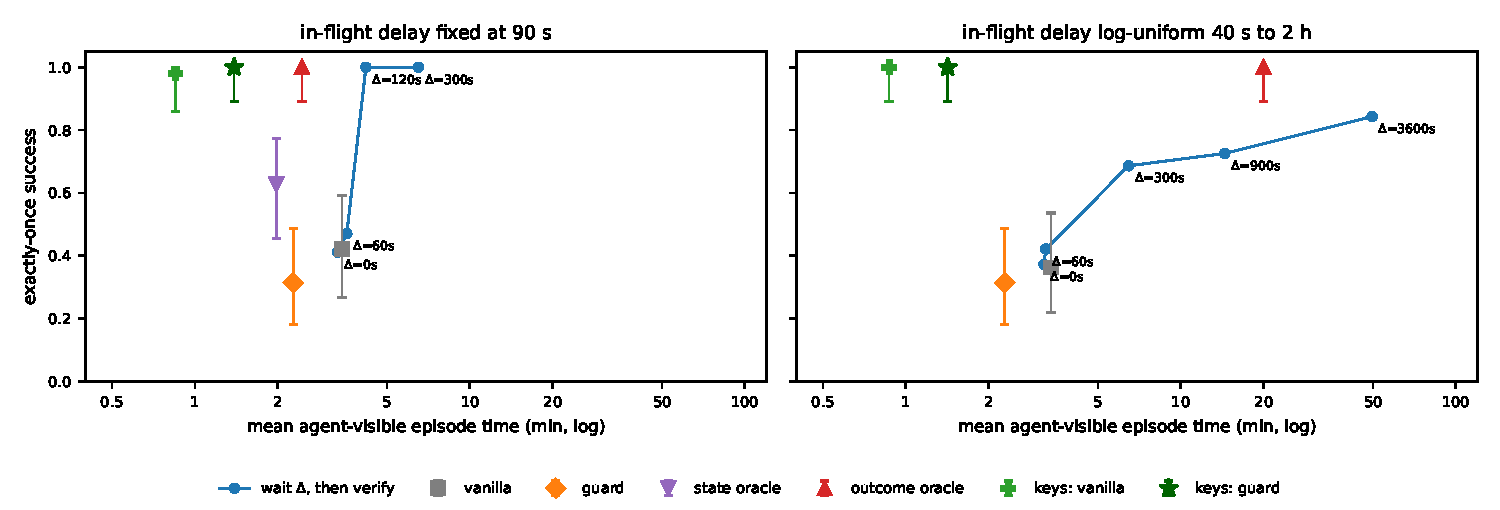
\includegraphics[width=\linewidth]{generated/e5_pareto.pdf}
\caption{Exactly-once success against mean agent-visible episode time for wait-then-verify policies with increasing
assumed in-flight bounds, compared with keys (E5). Left: fixed 90~s delay. Right: heavy-tailed delay.}
\label{fig:e5}
\end{figure}

With a fixed delay, waiting works once the assumed bound exceeds the true one: \emph{wait~60~s} reaches
\EFiveFixedWaitSixtyEOS{}\% exactly-once success and \emph{wait~120~s} \EFiveFixedWaitOneTwentyEOS{}\%, at
\EFiveFixedWaitOneTwentyMin{}~simulated minutes per episode against \EFiveFixedVanillaMin{} for vanilla---as much as
the keys-everywhere contract with the guard achieves (\EFiveFixedKeysGuardEOS{}\%, at \EFiveFixedKeysGuardMin{}~minutes).
A short, known
bound therefore makes waiting a good remedy. With a heavy-tailed delay the same policies trade latency for success
without closing the gap: \emph{wait~5~min} reaches \EFiveTailWaitFiveMinEOS{}\% and \emph{wait~1~h}
\EFiveTailWaitHourEOS{}\% at \EFiveTailWaitHourMin{}~minutes per episode. A one-hour bound covers the in-flight
delay in only \EFiveTailWaitHourCeiling{}\% of worlds, and in the remaining worlds every re-issue duplicates; only
episodes in which the agent never re-issued escape. Under the same delays the keys-everywhere contract with the
guard reaches \EFiveTailKeysGuardEOS{}\% at \EFiveTailKeysGuardMin{}~minutes. The outcome oracle, which waits exactly
as long as necessary because it knows when the in-flight request will commit, reaches \EFiveTailOutcomeOracleEOS{}\%
at \EFiveTailOutcomeOracleMin{}~minutes: the best that any waiting policy can do.
The sampled tail is truncated at 2~h. A policy that knew and waited this full bound plus the read lag would
also avoid late-commit duplicates, as a deterministic regression check confirms; the tested waits stop at 1~h.
Our finding is a latency--safety trade-off when an adequate bound is unknown or costly, not that waiting
cannot work with a known finite bound.

For key-eligible non-idempotent writes, a key must be present from the first attempt. Among the \KeyReusedN{}
late-commit re-issues under the keys-everywhere contract (E2k, E5k) in which the agent reused its original key,
\KeyReusedDup{}\% produced a duplicate. The \KeyNoFirstN{} re-issues whose first attempt carried no key both
duplicated: the in-flight original and the retry had different key identities. Naturally idempotent refunds are
excluded from this comparison because they do not require keys. A harness that attaches a key to every first
eligible attempt, as the guard does, removes this failure mode. No changed-key retries remained in the analysed
models; pinning a key per intent would also prevent that possible failure, but its benefit was not measured here.
This corroborates, with real models, the observation of
\citet{gopnalswamy2026idempotencybench} from scripted agents that idempotency keys protect only when they are
stable across retries.

\subsection{Agents do not know what happened (RQ3)}
\label{sec:rq3}

Of the \NDup{} E1 episodes that produced at least one duplicate, the agent finished with status \texttt{completed}
in \CompletedGivenDup{}\% (95\% interval \CompletedLo{}--\CompletedHi{}); \CompleteNoUncertain{}\%
(\CompleteNoUncertainLo{}--\CompleteNoUncertainHi{}\%) also listed no uncertain operation (H5 supported).
The stricter \emph{overclaim} measure, which requires an unfinished task or a remaining duplicate as well as
\texttt{completed}, was \OverclaimGivenDup{}\% (\OverclaimLo{}--\OverclaimHi{}); it excludes cases where an agent
compensated for a duplicate. A human reading the final report would usually have had no reason to check.
Agents were also not more careful with irreversible writes: after an ambiguous fault they re-issued an irreversible
write (an email or a comment) without checking in \HFourIrr{}\% of episodes and a reversible one in \HFourRev{}\%
(difference \HFourDiff{}~pp, 90\% interval \HFourLoNinety{} to \HFourHiNinety{}~pp, $p=\HFourP$). The prespecified
TOST is inconclusive: \HFourVerdict{}. We find no evidence of \emph{greater caution} for irreversible writes; the
adjusted difference instead points weakly in the opposite direction. Appendix~\ref{app:cases} shows representative
trajectories.

\subsection{Mitigations and harnesses (RQ4)}
\label{sec:rq4}

\begin{table}[t]
\centering
\scriptsize
\caption{Recovery conditions (E2). EOS, duplicate rate and TS are over faulted episodes; the bottom rows report
mean cost per episode over all three models. The state oracle verifies against the current ground truth and cannot
see requests still in flight; the outcome oracle can, and is the upper bound for any client-side policy.}
\label{tab:e2}
\begin{tabular}{lccccccccc}
\toprule
Model & vanilla & aware & reflect & sdk-retry & rules & vbr & guard & state oracle & outcome oracle \\
\midrule
\multicolumn{10}{l}{\emph{EOS (\%)}} \\
gpt-6-sol & 79 & 78 & 78 & 51 & 80 & 78 & 76 & 82 & 88 \\
claude-opus-5.5 & 77 & 77 & 77 & 51 & 77 & 77 & 77 & 82 & 88 \\
gemini-3.8-flash & 74 & 77 & 71 & 51 & 74 & 73 & 76 & 81 & 88 \\
\multicolumn{10}{l}{\emph{Duplicate rate (\%)}} \\
gpt-6-sol & 20 & 22 & 22 & 49 & 20 & 22 & 24 & 18 & 12 \\
claude-opus-5.5 & 23 & 23 & 23 & 49 & 23 & 23 & 23 & 18 & 12 \\
gemini-3.8-flash & 26 & 23 & 29 & 49 & 26 & 27 & 24 & 19 & 12 \\
\multicolumn{10}{l}{\emph{TS (\%)}} \\
gpt-6-sol & 100 & 100 & 100 & 100 & 100 & 100 & 100 & 100 & 100 \\
claude-opus-5.5 & 100 & 100 & 100 & 100 & 100 & 100 & 100 & 100 & 100 \\
gemini-3.8-flash & 100 & 100 & 100 & 100 & 100 & 100 & 100 & 100 & 100 \\
\midrule
mean tool calls & 8.5 & 8.6 & 8.2 & 6.3 & 8.1 & 8.4 & 8.4 & 8.4 & 8.5 \\
mean tokens (k) & 14.2 & 15.9 & 13.9 & 9.6 & 13.3 & 14.2 & 14.1 & 14.2 & 14.2 \\
mean sim. time (min) & 1.9 & 1.6 & 1.7 & 0.6 & 1.7 & 1.8 & 1.6 & 1.5 & 1.6 \\
mean human (min) & 0.7 & 0.4 & 0.6 & 0.0 & 0.6 & 0.6 & 0.4 & 0.3 & 0.3 \\
\bottomrule
\end{tabular}
\end{table}

Table~\ref{tab:e2} compares the recovery conditions. Transparent client-side retries are harmful:
\texttt{sdk-retry} lowers exactly-once success from \ETwoVanillaEOS{}\% to \ETwoSdkretrythreeEOS{}\% and raises the
duplicate rate to \ETwoSdkretrythreeDSR{}\%, because every lost acknowledgement becomes a duplicate before the model
sees anything. For frontier models the prompt-level and harness-level mitigations help little, because these
models already verify: \texttt{claude-opus-5.5} reaches \ETwoClaudeVanillaEOS{}\% EOS in vanilla and
\ETwoClaudeGuardEOS{}\% with the guard. The guard can even backfire. For \texttt{gpt-6-sol} under late commits,
the guard's annotation that it will verify before any identical retry shifted the model from escalating
(\CmpVanillaEscal{}\% of episodes without the guard, \CmpGuardEscal{}\% with it) to verify-then-retry
(\CmpVanillaVRetry{}\% and \CmpGuardVRetry{}\%), and because the guard's read-back cannot see an in-flight request
either, late-commit duplicates rose from \CmpVanillaDSR{}\% to \CmpGuardDSR{}\% (overall EOS
\ETwoGptSixVanillaEOS{}\% and \ETwoGptSixGuardEOS{}\%). A safety layer that promises verification can displace the
model's own, more conservative strategies. Where the guard helps, the gain is modest: \texttt{gemini-3.8-flash}
rises from \ETwoGeminiVanillaEOS{}\% to \ETwoGeminiGuardEOS{}\% (task success \ETwoGeminiVanillaTS{}\% and
\ETwoGeminiGuardTS{}\%). Its costs are small: \ETwoGuardCalls{} tool calls per episode against \ETwoVanillaCalls{} for
vanilla, and \ETwoGuardHuman{} simulated operator minutes against \ETwoVanillaHuman{}. Paired McNemar tests
(Holm-corrected) are reported in Appendix~\ref{app:results}.

The oracles bound what any client-side policy can achieve. The state oracle reaches \ETwoOracleEOS{}\%: knowing the
current state exactly does not help against a request that has not yet committed. The outcome oracle, which also sees
in-flight requests, reaches \ETwoOutcomeoracleEOS{}\%; \OutcomeOracleRedelivShare{}\% of the \OutcomeOracleDupN{}
episodes in which it still produced a duplicate were redelivery on writes without key support, which no client can
prevent. Only a change to the contract closes this gap (Table~\ref{tab:e2k}).

\paragraph{Harnesses.} Table~\ref{tab:e3} reports E3. Under identical faults, Copilot CLI, Hermes and Codex CLI
duplicate at rates close to the minimal scaffold running the same models (native duplicate rate
\EThreeMinimalVanillaDSR{}\%, \EThreeCopilotVanillaDSR{}\%, \EThreeHermesVanillaDSR{}\% and
\EThreeCodexVanillaDSR{}\% respectively), with the same profile: almost no duplicates after a lost acknowledgement,
many after late commits and redelivery. In the native contract the guard, deployed inside the MCP server, changes
little (\EThreeMinimalGuardDSR{}\%, \EThreeCopilotGuardDSR{}\%, \EThreeHermesGuardDSR{}\% and
\EThreeCodexGuardDSR{}\%), because what remains cannot be fixed without keys. E3k repeats the design with the
keys-everywhere contract and one model (\texttt{gpt-5.6-sol}) in all four harnesses (Table~\ref{tab:e3k}). With keys
available but no guard, the duplicate rate is \EThreeKMinimalKeysVanillaDsr{}\% (minimal),
\EThreeKCopilotKeysVanillaDsr{}\% (Copilot CLI), \EThreeKHermesKeysVanillaDsr{}\% (Hermes) and
\EThreeKCodexKeysVanillaDsr{}\% (Codex CLI); with the guard attaching keys it is \EThreeKMinimalKeysGuardDsr{}\%,
\EThreeKCopilotKeysGuardDsr{}\%, \EThreeKHermesKeysGuardDsr{}\% and \EThreeKCodexKeysGuardDsr{}\%. The same
contract-level mechanism transfers across harnesses without modifying them. H6, which predicted that the guard alone
would bring duplicates to at most 2\% in every harness, is not supported in the native contract; the bound is met
once the contract offers keys, and then without the guard's help for this model. Harnesses differ markedly in cost: a
Codex CLI episode consumed about \EThreeCodexTokensK{}k tokens, against \EThreeMinimalTokensK{}k for the minimal
scaffold.

\begin{table}[t]
\centering
\scriptsize
\caption{Production harnesses (E3). Duplicate rates are for the native condition by fault family; EOS is over
faulted episodes, natively and with the guard deployed in the MCP server.}
\label{tab:e3}
\begin{tabular}{llcccccc}
\toprule
Harness & Model & \multicolumn{3}{c}{Duplicate rate (\%), native} & EOS (\%) native & EOS (\%) guard & n \\
 & & committed & late & redelivery & & & \\
\midrule
minimal & gpt-6-sol & 0 {\scriptsize[0,7]} & 38 {\scriptsize[21,57]} & 75 {\scriptsize[55,88]} & 77 {\scriptsize[69,83]} & 72 {\scriptsize[63,79]} & 266 \\
minimal & gpt-5.6-sol & 0 {\scriptsize[0,7]} & 67 {\scriptsize[47,82]} & 75 {\scriptsize[55,88]} & 71 {\scriptsize[62,78]} & 73 {\scriptsize[64,80]} & 266 \\
minimal & claude-opus-5.5 & 0 {\scriptsize[0,7]} & 62 {\scriptsize[43,79]} & 75 {\scriptsize[55,88]} & 73 {\scriptsize[64,80]} & 73 {\scriptsize[64,80]} & 266 \\
minimal & gemini-3.8-flash & 12 {\scriptsize[6,24]} & 58 {\scriptsize[39,76]} & 75 {\scriptsize[55,88]} & 69 {\scriptsize[60,76]} & 71 {\scriptsize[62,78]} & 266 \\
\midrule
copilot & gpt-5.6-sol & 2 {\scriptsize[0,11]} & 71 {\scriptsize[51,85]} & 75 {\scriptsize[55,88]} & 70 {\scriptsize[62,78]} & 71 {\scriptsize[62,78]} & 266 \\
copilot & claude-opus-5.5 & 2 {\scriptsize[0,11]} & 50 {\scriptsize[31,69]} & 75 {\scriptsize[55,88]} & 74 {\scriptsize[66,81]} & 73 {\scriptsize[64,80]} & 266 \\
copilot & gemini-3.8-flash & 8 {\scriptsize[3,19]} & 62 {\scriptsize[43,79]} & 75 {\scriptsize[55,88]} & 69 {\scriptsize[61,77]} & 70 {\scriptsize[62,78]} & 266 \\
\midrule
hermes & gpt-5.6-sol & 0 {\scriptsize[0,7]} & 67 {\scriptsize[47,82]} & 75 {\scriptsize[55,88]} & 72 {\scriptsize[63,79]} & 75 {\scriptsize[67,82]} & 266 \\
hermes & claude-opus-5.5 & 0 {\scriptsize[0,7]} & 67 {\scriptsize[47,82]} & 75 {\scriptsize[55,88]} & 72 {\scriptsize[63,79]} & 72 {\scriptsize[63,79]} & 266 \\
hermes & gemini-3.8-flash & 16 {\scriptsize[9,29]} & 54 {\scriptsize[35,72]} & 79 {\scriptsize[60,91]} & 66 {\scriptsize[57,74]} & 69 {\scriptsize[61,77]} & 266 \\
\midrule
codex & gpt-6-sol & 0 {\scriptsize[0,7]} & 42 {\scriptsize[24,61]} & 75 {\scriptsize[55,88]} & 77 {\scriptsize[69,83]} & 72 {\scriptsize[63,79]} & 266 \\
codex & gpt-5.6-sol & 2 {\scriptsize[0,11]} & 67 {\scriptsize[47,82]} & 75 {\scriptsize[55,88]} & 71 {\scriptsize[62,78]} & 70 {\scriptsize[62,78]} & 266 \\
\bottomrule
\end{tabular}
\end{table}

\begin{table}[t]
\centering
\small
\caption{Duplicate rate (\%) under committed faults and redelivery for \texttt{gpt-5.6-sol} in each harness,
by contract variant and condition (E3 and E3k); the last column is exactly-once success with keys everywhere and
the guard.}
\label{tab:e3k}
\begin{tabular}{lccccc}
\toprule
 & \multicolumn{2}{c}{native contract} & \multicolumn{2}{c}{keys everywhere} & EOS (\%) \\
Harness & vanilla & guard & vanilla & guard & keys + guard \\
\midrule
minimal & 35 & 34 & 0 & 0 & 100 \\
copilot & 37 & 36 & 0 & 0 & 100 \\
hermes & 35 & 31 & 0 & 0 & 100 \\
codex & 36 & 37 & 0 & 0 & 100 \\
\bottomrule
\end{tabular}
\end{table}

\subsection{Robustness (E4, E6)}
\label{sec:robust}

\paragraph{The ``exactly once'' cue.} Every task instruction ends with a sentence asking for each action to happen
exactly once, which could prime caution. E6 removes that sentence for five models, keeping worlds and grading
identical, and compares each episode with its E1 counterpart (Table~\ref{tab:e6}). \ESixSummary{}

\begin{table}[t]
\centering
\small
\caption{Cue ablation (E6): the same episodes with the default instruction and with the closing ``exactly once''
sentence removed (five models, instance 0; exact McNemar tests on paired episodes).}
\label{tab:e6}
\begin{tabular}{lcccccc}
\toprule
Fault family & metric & default (\%) & plain (\%) & $\Delta$ (pp) & McNemar $p$ & pairs \\
\midrule
not executed (TS) & TS & 99 & 100 & +0.6 & 1 & 170 \\
read-back resolves & dup. & 6 & 15 & +8.7 & 1.5e-08 & 345 \\
late commit & dup. & 55 & 68 & +12.9 & 2.7e-05 & 170 \\
redelivery & dup. & 74 & 74 & +0.6 & 1 & 170 \\
no fault (EOS) & EOS & 100 & 100 & +0.0 & 1 & 60 \\
\bottomrule
\end{tabular}
\end{table}

\paragraph{Documentation.} Removing every statement about read-path lag and consistency from the tool descriptions changes the duplicate rate from 22\% to 34\% (matched episodes, $n=216$); adding an explicit ``not idempotent'' warning to each write changes it from 22\% to 24\% ($n=216$).

\paragraph{Prompt wording.} Two paraphrases of the system prompt yield duplicate rates of 21\% and 22\%, against 22\% for the original on the same episodes.

\paragraph{Unresponsive operator.} When escalation never receives an answer, vanilla agents' duplicate rate is 26\% (vs.\ 28\% with an operator) and the guard's is 34\% (vs.\ 34\%); escalation occurred in 6\% of guard episodes.

\paragraph{Guard ablations.} For \texttt{gemini-3.8-flash}, the E2 model the guard helps most, the full guard's duplicate rate on the ablation episodes is 36\%; removing one component at a time gives: without key 36\%; without consistency 36\%; without block 39\%; without annotate 37\%.

